\documentclass[aspectratio=169, 10pt]{beamer}

\usetheme[progressbar=frametitle, sectionpage=progressbar, numbering=fraction]{metropolis}

\usepackage{FiraSans}
\usepackage{FiraMono}
\usepackage{tikz}
\usetikzlibrary{arrows.meta, positioning, shapes.geometric, fit, backgrounds, decorations.pathreplacing}
\usepackage{xcolor}
\usepackage{fontawesome5}
\usepackage{booktabs}
\usepackage{array}
\usepackage{tcolorbox}
\tcbuselibrary{skins, breakable}

% ── Palette ─────────────────────────────────
\definecolor{charcoal}{HTML}{1C2541}
\definecolor{steel}{HTML}{3A506B}
\definecolor{sky}{HTML}{5BC0EB}
\definecolor{mint}{HTML}{C3E8BD}
\definecolor{offwhite}{HTML}{F5F5F5}
\definecolor{muted}{HTML}{8899AA}
\definecolor{danger}{HTML}{E84855}
\definecolor{yellow}{HTML}{F4D35E}

\setbeamercolor{normal text}{fg=charcoal, bg=white}
\setbeamercolor{alerted text}{fg=sky}
\setbeamercolor{example text}{fg=steel}

\setbeamercolor{frametitle}{bg=charcoal, fg=white}
\setbeamercolor{progress bar}{fg=sky, bg=charcoal!30}
\setbeamercolor{title separator}{fg=sky}

\setbeamercolor{block title}{bg=steel, fg=white}
\setbeamercolor{block body}{bg=offwhite, fg=charcoal}

\setbeamercolor{section in toc}{fg=charcoal}
\setbeamercolor{subsection in toc}{fg=steel}

% ── tcolorbox styles ────────────────────────
\tcbset{
  featurebox/.style={
    enhanced, colback=offwhite, colframe=steel,
    colbacktitle=steel, coltitle=white,
    fonttitle=\small\bfseries,
    boxrule=0.6pt, arc=4pt,
    top=4pt, bottom=4pt, left=6pt, right=6pt,
    attach boxed title to top left={yshift=-2mm, xshift=4mm},
    boxed title style={arc=2pt, boxrule=0pt},
  },
  statbox/.style={
    enhanced, colback=charcoal!6, colframe=charcoal!20,
    boxrule=0.5pt, arc=3pt,
    top=3pt, bottom=3pt, left=5pt, right=5pt,
    fontupper=\small,
  },
  codebox/.style={
    enhanced, colback=charcoal, colframe=charcoal,
    coltext=offwhite,
    boxrule=0pt, arc=4pt,
    top=5pt, bottom=5pt, left=8pt, right=8pt,
    fontupper=\ttfamily\small,
  },
}

\setbeamertemplate{navigation symbols}{}

% ─────────────────────────────────────────────
\title{\textbf{Your Agents}}
\subtitle{A Crewed-Agent AI Chat Platform}
\author{}
\date{}
% ─────────────────────────────────────────────

\begin{document}

% ── Title ────────────────────────────────────
{
\setbeamercolor{background canvas}{bg=charcoal}
\begin{frame}[plain, noframenumbering]
  \begin{tikzpicture}[remember picture, overlay]
    % Geometric accent shapes
    \fill[sky, opacity=0.15] (current page.south east) circle (5cm);
    \fill[sky, opacity=0.08] (current page.north west) circle (3.5cm);
    \fill[steel, opacity=0.2] ([xshift=2cm, yshift=-1cm]current page.north east) circle (4cm);

    % Content
    \node[anchor=west, text=white] at ([xshift=1.5cm, yshift=0.8cm]current page.west) {
      \begin{minipage}{0.65\textwidth}
        {\color{sky}\rule{1.2cm}{2pt}}\\[0.6em]
        {\fontsize{28}{34}\bfseries\color{white} Your Agents}\\[0.3em]
        {\large\color{offwhite!80!charcoal} A Crewed-Agent AI Chat Platform}
      \end{minipage}
    };

    % Right side decorative tag
    \node[anchor=east, text=muted] at ([xshift=-1.2cm, yshift=-0.5cm]current page.east) {
      \begin{minipage}{0.28\textwidth}
        \raggedleft
        {\small\color{muted}
          MCP Tools\\
          Knowledge Base\\
          Agent Observability\\
          Privacy by Design
        }
      \end{minipage}
    };
  \end{tikzpicture}
\end{frame}
}

% ── Table of Contents ────────────────────────
\begin{frame}{Agenda}
  \setbeamertemplate{section in toc}[sections numbered]
  \tableofcontents
\end{frame}

% ═══════════════════════════════════════════
\section{Overview}
% ═══════════════════════════════════════════

\begin{frame}{What is Your Agents?}
  \begin{columns}[T]
    \begin{column}{0.54\textwidth}
      \vspace{0.2em}
      {\large\bfseries A privacy-first AI chat platform}\\[0.5em]
      \small
      Users bring their own API keys and converse with LLMs through
      \textbf{OpenRouter} or \textbf{OpenAI}. Every request is enriched by a
      three-layer pipeline: knowledge retrieval, MCP tool execution, and
      streaming LLM completion — all orchestrated client-side.

      \vspace{1em}
      \begin{tcolorbox}[statbox]
        \begin{tabular}{@{}ll@{}}
          \faLayerGroup\ \textbf{Framework} & Next.js 15 App Router \\
          \faAtom\ \textbf{UI}              & React 19, Tailwind CSS 4 \\
          \faCode\ \textbf{Language}        & TypeScript \\
          \faDatabase\ \textbf{Storage}     & IndexedDB + LocalStorage \\
          \faRobot\ \textbf{LLM API}        & OpenRouter / OpenAI \\
          \faTools\ \textbf{Tool Protocol}  & MCP over HTTP \\
        \end{tabular}
      \end{tcolorbox}
    \end{column}

  \end{columns}
\end{frame}

\begin{frame}{Design Goals}
  \begin{itemize}
    \setlength\itemsep{0.9em}
    \item[\textcolor{sky}{\faLockOpen}] \textbf{Client-first privacy} — API keys never leave the browser
    \item[\textcolor{sky}{\faCogs}] \textbf{Extensible agent configuration} — system prompts, models, and tools per agent
    \item[\textcolor{sky}{\faEye}] \textbf{Observable agentic execution} — live reasoning, task list, and tool call results
    \item[\textcolor{sky}{\faHistory}] \textbf{Persistent sessions} — full chat history stored locally in IndexedDB
    \item[\textcolor{sky}{\faPlug}] \textbf{Pluggable MCP tool ecosystem} — SQL, LMS, Image, Browser connectors
  \end{itemize}
\end{frame}

% ═══════════════════════════════════════════
\section{Features}
% ═══════════════════════════════════════════

\begin{frame}{Features}
  \begin{columns}[T]
    \begin{column}{0.31\textwidth}
      \begin{tcolorbox}[featurebox, title={\faRobot\ \ Agent Management}]
        \scriptsize
        Create agents with distinct system prompts, model choices, and tool
        configs.\\[4pt]
        Import / export via JSON for easy sharing.
      \end{tcolorbox}\vspace{0.4em}

      \begin{tcolorbox}[featurebox, title={\faTools\ \ MCP Tool Execution}]
        \scriptsize
        Built-in connectors:\\[2pt]
        \textbullet\ \textbf{MySQL} — read-only SQL\\
        \textbullet\ \textbf{LMS} — Canvas, Brightspace, Blackboard\\
        \textbullet\ \textbf{Image} — gen \& processing\\
        \textbullet\ \textbf{Browser} — scraping \& automation
      \end{tcolorbox}
    \end{column}

    \begin{column}{0.31\textwidth}
      \begin{tcolorbox}[featurebox, title={\faBook\ \ Knowledge Management}]
        \scriptsize
        Per-agent knowledge store with custom generation prompts.
        Relevant entries are semantically retrieved and injected on every
        request.
      \end{tcolorbox}\vspace{0.4em}

      \begin{tcolorbox}[featurebox, title={\faChartBar\ \ Observability}]
        \scriptsize
        Live sidebar shows:\\[2pt]
        \textbullet\ Planner reasoning\\
        \textbullet\ Task list\\
        \textbullet\ Tool calls + raw results\\[4pt]
        Historical runs replayed from saved snapshots.
      \end{tcolorbox}
    \end{column}

    \begin{column}{0.31\textwidth}
      \begin{tcolorbox}[featurebox, title={\faHistory\ \ Session Management}]
        \scriptsize
        Named chat sessions in IndexedDB. Auto-generated titles via LLM.
        Full message history with per-message cost tracking.
      \end{tcolorbox}\vspace{0.4em}

      \begin{tcolorbox}[featurebox, title={\faMobile\ \ PWA Support}]
        \scriptsize
        Installable as a native-like app on any device. Supports web push
        notifications via VAPID and works offline for cached sessions.
      \end{tcolorbox}
    \end{column}
  \end{columns}
\end{frame}

\begin{frame}{Privacy Features}
  \begin{columns}[T]
    \begin{column}{0.48\textwidth}
      \begin{tcolorbox}[featurebox, title={\faKey\ \ User-provided API Keys}]
        \scriptsize
        No vendor lock-in. Users supply their own OpenRouter or OpenAI key.
        Keys are stored exclusively in \texttt{localStorage} — the server
        never sees them.
      \end{tcolorbox}\vspace{0.5em}

      \begin{tcolorbox}[featurebox, title={\faArrowsAltH\ \ Client-side API Calls}]
        \scriptsize
        All LLM requests travel \textbf{directly} from the browser to
        OpenRouter. No proxying through the application server — zero
        server-side logging of conversation content.
      \end{tcolorbox}\vspace{0.5em}

      \begin{tcolorbox}[featurebox, title={\faHdd\ \ Local Data Storage}]
        \scriptsize
        Chat history and agent configurations live in \textbf{IndexedDB}
        inside the user's browser. Nothing is synced to a backend database.
      \end{tcolorbox}
    \end{column}

    \begin{column}{0.48\textwidth}
      \begin{tcolorbox}[featurebox, title={\faServer\ \ No Server Processing}]
        \scriptsize
        The Next.js server only serves static assets and MCP tool endpoints.
        It does not process, store, or log any user messages or API
        responses.
      \end{tcolorbox}\vspace{0.5em}

      \begin{tcolorbox}[featurebox, title={\faShieldVirus\ \ Secured Tools}]
        \scriptsize
        MCP tool endpoints enforce strict safety guarantees:\\[3pt]
        \textbullet\ MySQL access is \textbf{read-only} only\\
        \textbullet\ Sensitive fields are \textbf{masked} in results\\
        \textbullet\ Row count capped at \textbf{20} by default\\
        \textbullet\ Credentials never appear in API responses
      \end{tcolorbox}
    \end{column}
  \end{columns}
\end{frame}

% ═══════════════════════════════════════════
\section{Architecture}
% ═══════════════════════════════════════════

\begin{frame}{Core Components}
  \begin{center}
  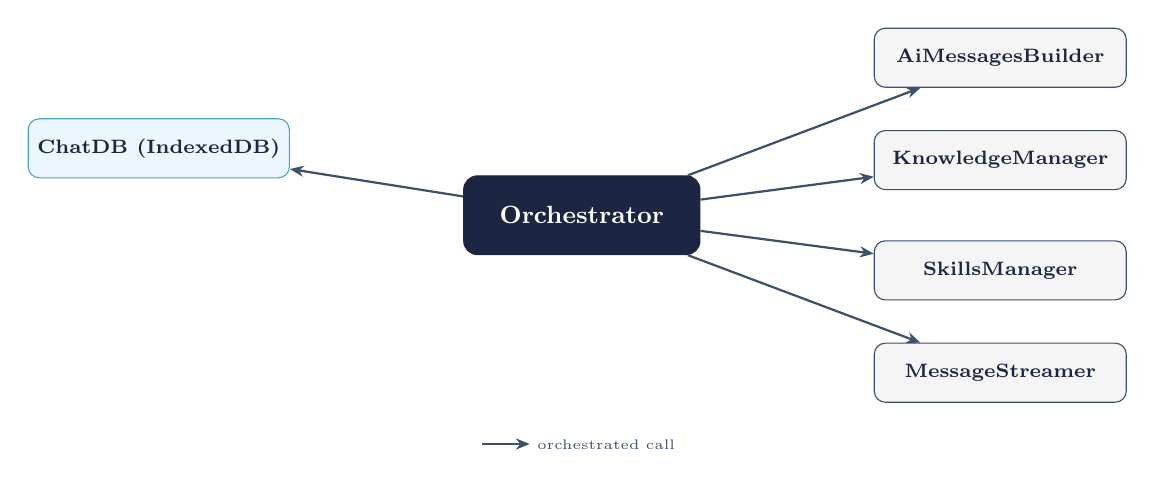
\begin{tikzpicture}[
    node distance=0.5cm and 2.0cm,
    orch/.style={rectangle, rounded corners=5pt,
                 draw=charcoal, fill=charcoal, text=white,
                 minimum width=3cm, minimum height=1cm,
                 font=\small\bfseries, align=center},
    comp/.style={rectangle, rounded corners=4pt,
                 draw=steel, fill=offwhite, text=charcoal,
                 minimum width=3.2cm, minimum height=0.75cm,
                 font=\scriptsize\bfseries, align=center},
    store/.style={rectangle, rounded corners=4pt,
                  draw=sky!80!charcoal, fill=sky!12, text=charcoal,
                  minimum width=3.2cm, minimum height=0.75cm,
                  font=\scriptsize\bfseries, align=center},
    arr/.style={-{Stealth[length=5pt, width=4pt]}, thick, color=steel},
    darr/.style={-{Stealth[length=5pt, width=4pt]}, thick, color=sky, dashed},
  ]
    \node[orch] (orch) {Orchestrator};

    \node[comp, right=2.2cm of orch, yshift= 2.0cm] (amb) {AiMessagesBuilder};
    \node[comp, right=2.2cm of orch, yshift= 0.7cm] (km)  {KnowledgeManager};
    \node[comp, right=2.2cm of orch, yshift=-0.7cm] (sm)  {SkillsManager};
    \node[comp, right=2.2cm of orch, yshift=-2.0cm] (ms)  {MessageStreamer};

    \node[store, left=2.2cm of orch, yshift= 0.85cm] (db) {ChatDB (IndexedDB)};

    \foreach \t in {amb, km, sm, ms}
      \draw[arr] (orch) -- (\t);
    \foreach \t in {db}
      \draw[arr] (orch) -- (\t);

    % Legend
    \node[font=\tiny, text=steel, anchor=south west] at (-1.4,-3.1) {%
      \tikz\draw[arr](-0.2,0)--(0.4,0); orchestrated call};
  \end{tikzpicture}
  \end{center}
\end{frame}

\begin{frame}{Message Flow}
  \begin{center}
  \begin{tikzpicture}[
    node distance=0.32cm,
    sbox/.style={rectangle, rounded corners=3pt,
                 draw=charcoal!40, fill=charcoal!6,
                 minimum width=11cm, minimum height=0.62cm,
                 font=\scriptsize\bfseries, text=charcoal, align=left,
                 inner sep=7pt},
    obox/.style={rectangle, rounded corners=3pt,
                 draw=sky!60, fill=sky!8,
                 minimum width=11cm, minimum height=0.62cm,
                 font=\scriptsize\itshape, text=steel, align=left,
                 inner sep=7pt},
    arr/.style={-{Stealth[length=4pt]}, thick, color=charcoal!50},
    lbl/.style={font=\tiny\bfseries, text=sky},
  ]
    \node[sbox] (inp)    {\faUser\ \ \textbf{1.} User input — text or image (base64-encoded for vision models)};
    \node[sbox, below=of inp]    (build)  {\faList\ \ \textbf{2.} AiMessagesBuilder — sliding window of last 10 msgs + agent system prompt};
    \node[obox, below=of build]  (know)   {\faBook\ \ \textbf{3.} KnowledgeManager — semantic retrieval, inject as system message \emph{[if configured]}};
    \node[obox, below=of know]   (skill)  {\faTools\ \ \textbf{4.} SkillsManager — plan tasks, execute MCP tools, inject results \emph{[if enabled]}};
    \node[sbox, below=of skill]  (stream) {\faBolt\ \ \textbf{5.} MessageStreamer — streaming LLM call, token-by-token UI update};
    \node[sbox, below=of stream] (save)   {\faDatabase\ \ \textbf{6.} ChatDB — persist all messages + AgentRunSnapshot};

    \foreach \a/\b in {inp/build, build/know, know/skill, skill/stream, stream/save}
      \draw[arr] (\a) -- (\b);

    % Optional bracket
    \draw[sky, thick, decorate, decoration={brace, amplitude=5pt}]
      ([xshift=11.2cm]know.north east) -- ([xshift=11.2cm]skill.south east)
      node[midway, right=6pt, font=\tiny\itshape, text=sky] {optional};
  \end{tikzpicture}
  \end{center}
\end{frame}

\begin{frame}{SkillsManager — Internal Pipeline}
  \begin{center}
  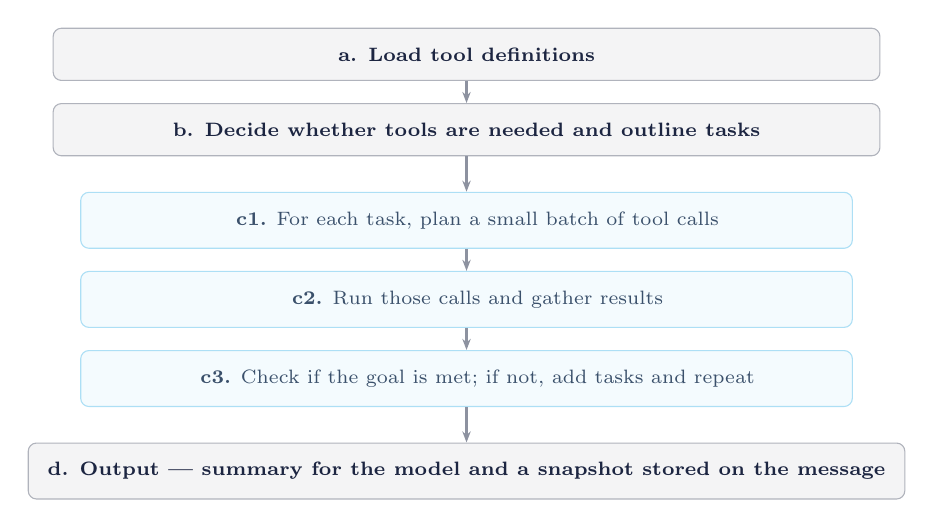
\begin{tikzpicture}[
    node distance=0.28cm,
    sbox/.style={rectangle, rounded corners=3pt,
                 draw=charcoal!35, fill=charcoal!5,
                 minimum width=10.5cm, minimum height=0.6cm,
                 font=\scriptsize\bfseries, text=charcoal, align=left, inner sep=7pt},
    lbox/.style={rectangle, rounded corners=3pt,
                 draw=sky!50, fill=sky!7,
                 minimum width=9.8cm, minimum height=0.6cm,
                 font=\scriptsize, text=steel, align=left, inner sep=7pt},
    arr/.style={-{Stealth[length=4pt]}, thick, color=charcoal!50},
    larr/.style={-{Stealth[length=4pt]}, thick, color=sky!70},
  ]
    \node[sbox] (schema) {\textbf{a.} Load tool definitions};
    \node[sbox, below=of schema] (plan) {\textbf{b.} Decide whether tools are needed and outline tasks};

    \node[lbox, below=0.45cm of plan] (l1) {\quad\textbf{c1.} For each task, plan a small batch of tool calls};
    \node[lbox, below=of l1]          (l2) {\quad\textbf{c2.} Run those calls and gather results};
    \node[lbox, below=of l2]          (l3) {\quad\textbf{c3.} Check if the goal is met; if not, add tasks and repeat};

    \node[sbox, below=0.45cm of l3] (out) {\textbf{d.} Output — summary for the model and a snapshot stored on the message};

    % loop brace
    \draw[arr] (schema) -- (plan);
    \draw[arr] (plan)   -- (l1);
    \draw[arr] (l1)     -- (l2);
    \draw[arr] (l2)     -- (l3);
    \draw[arr] (l3)     -- (out);
  \end{tikzpicture}
  \end{center}
\end{frame}

% ═══════════════════════════════════════════
\section{Privacy \& Security}
% ═══════════════════════════════════════════

\begin{frame}{Privacy \& Security}
  \begin{columns}[T]
    \begin{column}{0.46\textwidth}
      \begin{tcolorbox}[featurebox, title={\faLaptop\ \ Client-side guarantees}]
        \scriptsize
        \begin{itemize}
          \setlength\itemsep{3pt}
          \item API keys stored only in \texttt{localStorage}
          \item Chat history \& Agent configs lives in IndexedDB, never sent to the server
          \item LLM calls \textbf{directly} from browser $\to$ OpenRouter
        \end{itemize}
      \end{tcolorbox}

      \vspace{0.5em}

      \begin{tcolorbox}[featurebox, title={\faServer\ \ Server-side guarantees}]
        \scriptsize
        \begin{itemize}
          \setlength\itemsep{3pt}
          \item MySQL MCP is \textbf{read-only} — only \texttt{SELECT}, \texttt{SHOW}, \texttt{DESCRIBE}
          \item Sensitive fields masked in all query results
          \item \texttt{LIMIT} enforced on each query (20 rows)
        \end{itemize}
      \end{tcolorbox}
    \end{column}

    \begin{column}{0.50\textwidth}
      \vspace{0.2em}
      {\small\bfseries Storage model}\\[0.5em]
      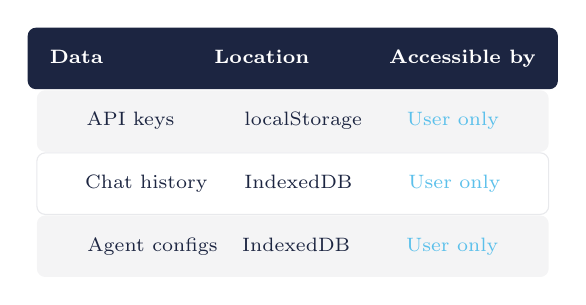
\begin{tikzpicture}[
        row/.style={rectangle, rounded corners=3pt,
                    minimum width=6.5cm, minimum height=0.65cm,
                    font=\scriptsize, align=left, inner sep=8pt},
        hdr/.style={row, fill=charcoal, text=white, font=\scriptsize\bfseries},
        odd/.style={row, fill=charcoal!5, text=charcoal},
        evn/.style={row, fill=white, text=charcoal, draw=charcoal!10},
        node distance=0pt,
      ]
        \node[hdr] (h) {Data \hspace{1.2cm} Location \hspace{0.8cm} Accessible by};
        \node[odd, below=of h]  (r1) {API keys \hspace{0.7cm} localStorage \hspace{0.38cm} \textcolor{sky}{User only}};
        \node[evn, below=of r1] (r2) {Chat history \hspace{0.28cm} IndexedDB \hspace{0.52cm} \textcolor{sky}{User only}};
        \node[odd, below=of r2] (r3) {Agent configs \hspace{0.12cm} IndexedDB \hspace{0.52cm} \textcolor{sky}{User only}};
      \end{tikzpicture}
    \end{column}
  \end{columns}
\end{frame}

% ── Closing ───────────────────────────────────
{
\setbeamercolor{background canvas}{bg=charcoal}
\setbeamercolor{normal text}{fg=white}
\begin{frame}[plain, noframenumbering, c]
  \centering
  {\color{sky}\rule{2cm}{2pt}}\\[1em]
  {\fontsize{32}{38}\bfseries\color{white} Thank You}\\[0.8em]
  {\large\color{offwhite!60!charcoal} Questions \& Discussion}
\end{frame}
}

\end{document}
